\documentclass[11pt]{article}


%use the english line for english reports
%usepackage[english]{babel}
\usepackage[portuguese]{babel}
\usepackage[utf8]{inputenc}
\usepackage{indentfirst}
\usepackage{graphicx}
\usepackage{verbatim}
\usepackage{textcomp}
\usepackage{listings}
\usepackage{color}


\begin{document}


\setlength{\textwidth}{16cm}
\setlength{\textheight}{22cm}

\title{\Huge\textbf{Protocolo de Ligação de Dados}\linebreak\linebreak\linebreak
\Large\textbf{Relatório do 1º trabalho laboratorial}\linebreak
\linebreak\linebreak

\includegraphics[scale=0.1]{feup-logo.png}\linebreak
\linebreak\linebreak
\Large{Mestrado Integrado em Engenharia Informática e Computação} \linebreak\linebreak
\Large{Redes de Computadores}
}

\author{\textbf{Grupo xx:}\\
Francisco Rodrigues - 201305627l\\
João Nogueira - 201303882 \\
Marta Lopes - 201208067 \\
\linebreak\linebreak \\
 \\ Faculdade de Engenharia da Universidade do Porto \\ Rua Roberto Frias, s\/n, 4200-465 Porto, Portugal \linebreak\linebreak\linebreak
\linebreak\linebreak\vspace{1cm}}

\maketitle
\thispagestyle{empty}

\newpage
\tableofcontents
\newpage

%************************************************************************************************
%************************************************************************************************

\newpage

%Todas as figuras devem ser referidas no texto. %\ref{fig:codigoFigura}
%
%%Exemplo de código para inserção de figuras
%%\begin{figure}[h!]
%%\begin{center}
%%escolher entre uma das seguintes três linhas:
%%\includegraphics[height=20cm,width=15cm]{path relativo da imagem}
%%\includegraphics[scale=0.5]{path relativo da imagem}
%%\includegraphics{path relativo da imagem}
%%\caption{legenda da figura}
%%\label{fig:codigoFigura}
%%\end{center}
%%\end{figure}
%
%
%\textit{Para escrever em itálico}
%\textbf{Para escrever em negrito}
%Para escrever em letra normal
%``Para escrever texto entre aspas''
%
%Para fazer parágrafo, deixar uma linha em branco.
%
%Como fazer bullet points:
%\begin{itemize}
	%\item Item1
	%\item Item2
%\end{itemize}
%
%Como enumerar itens:
%\begin{enumerate}
	%\item Item 1
	%\item Item 2
%\end{enumerate}
%
%\begin{quote}``Isto é uma citação''\end{quote}


%%%%%%%%%%%%%%%%%%%%%%%%%%
\section{Sumário}

Este relatório tem como objetivo explicar o primeiro projeto, realizado para esta unidade curricular, denominado "Protocolo de Ligação de Dados". Este projeto consiste no envio de informação de um computador para outro, através do uso de porta de série. Foram assim implementados programas para ler e escrever a informação a ser enviada.
\par O projeto foi finalizado com sucesso, sendo que os dados foram enviados e recebidos de forma correcta. Foram também incluídos a prevenção e correção de erros ao longo da transmissão, restabelecendo a transmissão quando os erros acontecem.


%%%%%%%%%%%%%%%%%%%%%%%%%%
\section{Introdução}

Iremos então descrever o nosso trabalho, que consiste em implementar um protocolo de  ligação de dados, de acordo com a especificação descrita no guião, de uma forma mais teórica e pormenorizada para assim poderem ser avaliados certos aspectos que não seriam possíveis avaliar durante a apresentação na aula. 
O ambiente de desenvolvimento utilizado foi em PC's com \textit{Linux}, a linguagem de programação foi C e as portas de série existentes realizavam comunicação assíncrona. 
\par O protocolo de  ligação de dados pretende assim fornecer um serviço de comunicação de dados fiável entre dois sistemas ligados por um cabo de série. As funções utilizadas serão a de criação e sincronismo de tramas que irão organizar os dados a ser enviados (\textit{framing}), a do estabelecimento/conclusão da ligação, a numeração de tramas, o controlo de fluxo, a confirmação de envio sem erros e o controlo dos erros que poderão ser criados por \textit{timeouts}, tramas fora da sequência esperada ou retransmissões. 
\par O nosso relatório terá então as \textbf{secções principais} seguintes:

\begin{itemize}
	\item \textbf{Arquitetura}: especificação dos blocos funcionais e da \textit{interface};
	\item \textbf{Estrutura do código}: API's, principais estruturas de dados, principais funções e a sua relação com a arquitetura;
	\item \textbf{Casos de uso principais}: identificar os principais aspectos, abordando as sequências de chamadas de funções;
	\item \textbf{Protocolo de ligação lógica}: identificar os principais aspectos funcionais da \textit{linkLayer}, descrevendo a estratégia de implementação;
	\item \textbf{Protocolo de aplicação}:  identificar os principais aspectos funcionais da \textit{applicationLayer}, descrevendo a estratégia de implementação;
	\item \textbf{Validação}: testes efetuados ao programa com apresentação de resultados;
	\item \textbf{Elementos de valorização}: identificação dos elementos implementados, descrevendo a estratégia de implementação.
\end{itemize}


%%%%%%%%%%%%%%%%%%%%%%%%%%
\section{Arquitetura}

\subsection{\textit{Application Layer} e \textit{Link Layer}}

O projeto está organizado em duas \textit{layers} que vão ser responsáveis pela correta funcionalidade do mesmo. A \textit{layer} que vai servir para a aplicação tem os ficheiros \textit{applicationLayer.c} e \textit{applicationLayer.h} e a ligação lógica está representada nos ficheiros \textit{linkLayer.c} e \textit{linkLayer.h} com um ficheiro *.h auxiliar, o \textit{linkLayerAux.h}.\newline

A \textbf{camada de ligação lógica}, contém várias funções, servindo estas para a configuração e abertura da porta de série, o envio de comandos, envio e receção de mensagens e para a realização dos processos de \textit{stuffing} e \textit{destuffing}.\newline

A \textbf{camada de aplicação}, que vai depender da camada de ligação lógica utilizando algumas das suas funções, disponibilizará funções onde serão especificados o envio e receção de pacotes de dados, o envio e receção de pacotes de controlo e finalmente a leitura e a escrita do ficheiro a enviar. 

\subsection{\textit{Interface}}

A interface na linha de comandos está implementada nos ficheiros \textit{cli.c} e \textit{cli.h} que têm as funções que vão permitir a escolha de valores de alguns parâmetros referentes à transferência do ficheiro, existindo limites impostos de acordo com o guião. 
Os parâmetros a serem especificados pelo utilizador serão a \textit{baudrate}, o tamanho máximo para a mensagem, o número de \textit{timeouts} máximo no caso de falha de comunicação e a duração de cada \textit{timeout}. Além disso, o utilizador terá também de dizer se será o transmissor ou o recetor e qual é a sua porta de série. Depois de o utilizador especificar cada um destes valores a aplicação vai iniciar, sendo que terá uma informação inicial mostrando os parâmetros com a escolha feita pelo utilizador. 


\newpage
%%%%%%%%%%%%%%%%%%%%%%%%%%
\section{Estrutura do código}

\subsection{Application Layer}
 
  A camada da aplicação está implementada nos ficheiro \textit{applicationLayer.c} e \textit{applicationLayer.h} e é representada por uma estrutura na qual se encontram um \textit{char} que representa o modo do programa (Receptor/Transmissor) e um inteiro chamado debug que permite fazer o \textit{debugging} através de prints ao longo do código.
 
\small
\lstset{frame=tb,
  language={[Visual]Basic},
  aboveskip=3mm,
  belowskip=3mm,
  showstringspaces=false,
  columns=flexible,
  basicstyle={\small\ttfamily},
  numbers=none,
  numberstyle=\tiny\color{gray},
  keywordstyle=\color{blue},
  commentstyle=\color{dkgreen},
  stringstyle=\color{mauve},
  breaklines=true,
  breakatwhitespace=true
  tabsize=3
}
\lstinputlisting{./code/struct1.c}
\normalsize

\subsection{Link Layer}
 
 É nos ficheiros \textit{linkLayer.c}, \textit{linkLayer.h} e \textit{linkLayerAux.h} que está implementada a camada de ligação de dados representada por uma estrutura na qual se encontram:

\begin{itemize}
  \item A porta de série;
   \item O Baud Rate;
   \item O número de sequência;
   \item O timeout;
   \item O número de tentativas;
   \item O tamanho máximo de cada pacote;
   \item Estrutura de estatísticas.
\end{itemize}

\small
\lstset{frame=tb,
  language={[Visual]Basic},
  aboveskip=3mm,
  belowskip=3mm,
  showstringspaces=false,
  columns=flexible,
  basicstyle={\small\ttfamily},
  numbers=none,
  numberstyle=\tiny\color{gray},
  keywordstyle=\color{blue},
  commentstyle=\color{dkgreen},
  stringstyle=\color{mauve},
  breaklines=true,
  breakatwhitespace=true
  tabsize=3
}
\lstinputlisting{./code/struct2.c}
\normalsize

\newpage
%%%%%%%%%%%%%%%%%%%%%%%%%%
\section{Casos de uso principais}

 (identificação; sequências de chamada de funções)

%%%%%%%%%%%%%%%%%%%%%%%%%%

\newpage
%%%%%%%%%%%%%%%%%%%%%%%%%%
\section{Protocolo de ligação lógica}

O protocolo de ligação lógica está implementado na camada \textit{linkLayer}, camada da qual depende a camada \textit{applicationLayer}.

\subsection{Principais aspectos funcionais}
\begin{itemize}
  \item Configurar a porta de série como é pretendido;
  \item Repor a configuração da porta de série como originalmente após a transferência dos dados pretendidos;
  \item  Estabelecer a ligação de dados utilizando a porta de série;
  \item  Enviar comandos;
  \item  Enviar/receber mensagens;
  \item Processo de \textit{Stuffing} e \textit{Destuffing} dos \textit{packets} recebidos da camada \textit{applicationLayer}.
\end{itemize}


\subsection{Funções implementadas na \textit{linkLayer}}
  
 \subsubsection{ll\_open}

	Esta função é responsável por configurar a porta de série com as opções pretendidas (utilizando, por exemplo, o \textit{baudRate} escolhido pelo utilizador) e por guardar numa variável que passa por argumento à função \textit{configure}.
	Depois de configurar a porta de série, do lado do emissor envia o comando SET e aguarda a resposta UA do recetor que, ao ser recebida termina a função. Utiliza o alarme para controlar os \textit{timeouts}. Do lado do recetor aguarda a recepção do comando SET e, ao recebê-lo responde com o comando UA.
   	
  \subsubsection{ll\_close}
   
    Do lado do receptor, esta função começa por aguardar a recepção do comando DISC, respondendo com o mesmo comando. Após o envio deste comando, e imediatamente antes de reestabelecer as configurações originais da porta de série aguarda a recepção do comando UA por parte do emissor.
	Do lado do emissor, esta função começa por enviar o comando DISC e aguarda pela resposta com o mesmo comando por parte do receptor (implementando o alarme para manter controlo dos timeouts). Após a correta recepção de DISC evia o último comando do programa, comando UA.
    Termina por fazer \textit{resetConfiguration}, função na qual é feito um \textit{sleep} de um segundo por forma a garantir que as configurações originais da porta de série não são restabelecidas antes de que toda a informação tenha sido passada.
   
 \subsubsection{llwrite}
    
	Esta função começa por alocar memória num \textit{buffer} no qual a informação será organizada (antes do processo de \textit{stuffing}). Após alocar a memória necessária começa por atribuir os valores de FLAG, A, C e BCC de acordo com o número de sequência da trama. A partir de BCC é copiada para o buffer toda a informação recebida por argumento desta função da \textit{applicationLayer} correspondente ao \textit{packet} a enviar. Antes de terminar o preenchimento do \textit{buffer} coloca o BCC2 ('ou' exclusivo dos octetos do \textit{packet}) e a FLAG para terminar.
	Depois de ter a trama preenchida e antes de começar o processo de envio, envia o \textit{buffer} para a função \textit{stuff} que retorna um \textit{buffer} com a trama pronta para envio.
	Envia a trama através da porta de série e aguarda a resposta por parte do recetor, o que vai determinar o caminho a seguir pela função, que pode variar entre terminar a função pois houve a recepção de RR, ou re-enviar a mesma trama por ter sido rejeitada.
	A mesma trama pode ser re-enviada por ocorrência de \textit{timeout}, o que também é controlado nesta função através da implementação de alarmes.
	Esta função pode também terminar pela ocorrência de \textit{timeouts} maior do que o número máximo definido previamente pelo utilizador.
	
 \subsubsection{llread}
   
    A função \textit{llread} começa por alocar memória para o \textit{buffer} que vai ser recebido, entrando imediatamente a seguir num ciclo do ual apenas sai quando algo é lido da porta de série.
	Após a leitura o \textit{buffer} lido é passado para a função responsável pelo processo de \textit{destuffing} que retorna a trama de Informação recebida "descodificada". 
	Os valores de BCC e de BCC2 são verificados por forma a garantir que a trama foi recebida sem erros, caso o tenha sido é interpretado o número de sequência e se tudo for o pretendido é enviado o comando RR, caso contrário é enviado o comando REJ, pedindo que a mesma seja enviada novamente.


%%%%%%%%%%%%%%%%%%%%%%%%%%

\newpage
%%%%%%%%%%%%%%%%%%%%%%%%%%
\section{Protocolo de aplicação}

O protocolo de aplicação está implementado na camada applicationLayer, camada esta que depende, como dito anteriormente, da camada linkLayer.

 \subsection{Principais aspectos funcionais}
 \begin{itemize}
  \item Envio e recepção de pacotes de dados;
  \item Envio e recepção de pacotes de controlo;
  \item Leitura do ficheiro a enviar;
  \item Escrita do ficheiro a enviar.
\end{itemize}
  
  \subsection{Funções implementadas na \textit{applicationLayer}}
	\textbf{main}
    
	Chama as diversas funções da \textit{Interface} do utilizador e recebe o seu \textit{input} por forma a inicializar o programa com as configurações desejadas pelo utilizador. Chama as funções \textit{ll\_open, ll\_close}, \textit{readFile} e \textit{sendFile}.\newline
	
   \textbf{initStat}
   
    Função responsável por inicializar os valores da estrutura de estatística. Esta estrutura é utilizada para que, no final da execução do programa, o utilizador esteja a par do que aconteceu no desenrolar do programa.\newline
	
  \textbf{fillLinkLayer}
   
    Função responsável por inicializar a estrutura\textit{ linkLayer}, estrutura essa passada para muitas das funções utilizadas ao longo do programa. Nesta estrutura estão atributos como por exemplo: \textit{baudRate, timeout}, etc.\newline
	
   \textbf{createFirstControlPacket}
   
    Função responsável por gerar o primeiro pacote de controlo. É colocado neste pacote o tamanho do ficheiro a enviar bem como o nome do mesmo.\newline
	
    \textbf{getNameAndSizeOfFile}
   
    Esta função é responsável por, dado o primeiro pacote de controlo recebido, interpretar qual o nome e tamanho do ficheiro a receber.\newline
	
   \textbf{sendFile}
   
    Esta função começa por ler toda a informação do ficheiro a enviar e guarda-a num \textit{buffer} de chars, \textit{buffer} a partir do qual a informação será lida para envio. Após a leitura chama a função responsável pelo envio do primeiro pacote de controlo e envia-o para o recetor chamando \textit{llwrite} (função do pacote de ligação). Depois do envio do primeiro pacote de controlo é calculado o número de pacotes necessários a enviar tendo em conta o tamanho máximo definido previamente pelo utilizador, e entra num ciclo que é percorrido o número de vezes igual ao número de pacotes de dados. Neste ciclo é, inicialmente criado o pacote de dados, com a informação necessária (C, número de sequência, número de octetos do campo de dados) e com os dados em si. É chamada a função \textit{llwrite} para enviar o pacote e repete-se o ciclo até ao final do envio dos dados (atualizando sempre a barra de progresso no ecrã).\newline
   
    \textbf{readFile}
   
    Esta é a função responsável pela recepção de todo o ficheiro e pela sua escrita em disco. Começa por entrar num ciclo que termina quando o último pacote de controlo é lido. Dentro do ciclo o primeiro passo é chamar a função \textit{llread }que retorna, após a leitura, o pacote a interpretar.
	São então tomadas medidas diferentes nos casos de ser o primeiro pacote de controlo, o último pacote de controlo ou um pacote de dados. No caso de ser o primeiro pacote de controlo é guardada a informação do nome e tamanho do ficheiro. No caso de ser o último pacote de controlo é criado o ficheiro e toda a informação lida, até agora guardada num\textit{ buffer}, é escrita em disco. No caso de ser um pacote de dados a informação é adicionada no final do \textit{buffer} de leitura.
	Sempre que um pacote é lido é atualizada a barra de progresso.\newline


%%%%%%%%%%%%%%%%%%%%%%%%%%

\newpage
%%%%%%%%%%%%%%%%%%%%%%%%%%
\section{Validação}

Para verificar se a transferência do ficheiro \textit{pinguim.gif} foi efetuada com sucesso decidimos colocar uma verificação de inicio e fim de envio,  durante o envio do ficheiro adicionamos uma barra de progresso que iria sendo actualizada à medida que os packets iam sendo enviados. 
\begin{figure}[h!]
\begin{center}
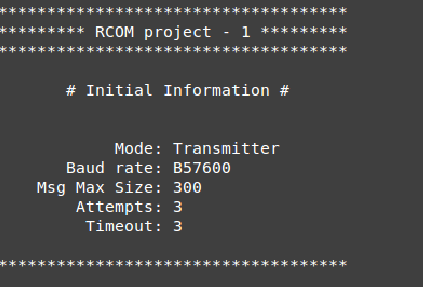
\includegraphics[scale=0.6]{trans1.png}
\caption{Informações iniciais - Modo Transmissor}
\label{fig:codigoFigura}
\end{center}
\end{figure}

\begin{figure}[h!]
\begin{center}
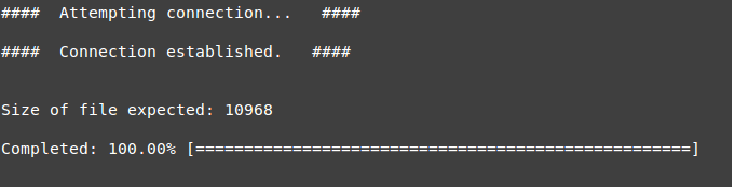
\includegraphics[scale=0.6]{trans2.png}
\caption{Inicio do envio e barra de progresso - Modo Transmissor}
\label{fig:codigoFigura}
\end{center}
\end{figure}

\begin{figure}[h!]
\begin{center}
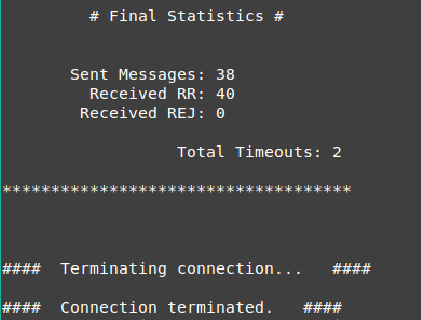
\includegraphics[scale=0.6]{trans3.png}
\caption{Fim do envio e estatisticas - Modo Transmissor}
\label{fig:codigoFigura}
\end{center}
\end{figure}

\begin{figure}[h!]
\begin{center}
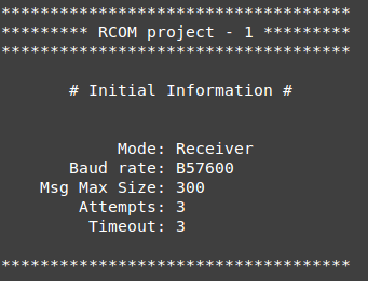
\includegraphics[scale=0.6]{rec1.png}
\caption{Informações iniciais - Modo Recetor}
\label{fig:codigoFigura}
\end{center}
\end{figure}

\begin{figure}[h!]
\begin{center}
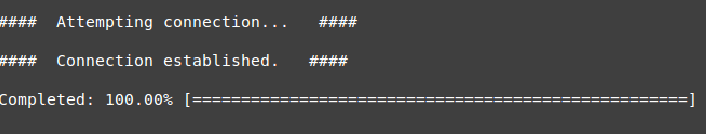
\includegraphics[scale=0.6]{rec2.png}
\caption{Inicio do envio e barra de progresso - Modo Recetor}
\label{fig:codigoFigura}
\end{center}
\end{figure}

\begin{figure}[h!]
\begin{center}
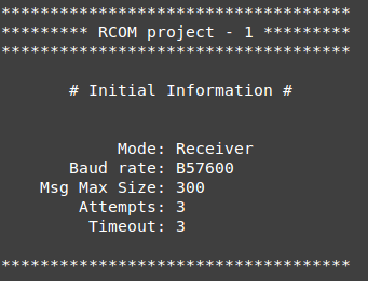
\includegraphics[scale=0.65]{rec1.png}
\caption{Fim do envio e estatisticas - Modo Recetor}
\label{fig:codigoFigura}
\end{center}
\end{figure}

Adicionamos também o modo \textit{debug} em que iriam ser feitos mais \textit{prints} à medida que o ficheiro ia sendo enviado, sendo também possível verificar quando houvesse \textit{timeouts} ou envio/receção de REJ's. 





%%%%%%%%%%%%%%%%%%%%%%%%%%

\newpage
%%%%%%%%%%%%%%%%%%%%%%%%%%
\section{ Elementos de valorização}
  (identificação dos elementos de valorização implementados; descrição da estratégia de implementação com apresentação de pequenos extratos de código) 


%%%%%%%%%%%%%%%%%%%%%%%%%%

\newpage
%%%%%%%%%%%%%%%%%%%%%%%%%%
\section{Conclusões}
 (síntese da informação apresentada nas secções anteriores; reflexão sobre os objectivos de aprendizagem alcançados)


%%%%%%%%%%%%%%%%%%%%%%%%%%

\newpage
%%%%%%%%%%%%%%%%%%%%%%%%%%
\section{Anexos}



%%%%%%%%%%%%%%%%%%%%%%%%%%

\end{document}
